\include{parameters}
\usetheme{AFNIC}
\usepackage[english]{babel}
\usepackage[latin1]{inputenc}
\usepackage{bortzmeyer-utils}

\title{DNSwitness: recent developments and the new passive monitor}
\author{St�phane Bortzmeyer\\AFNIC\\\texttt{bortzmeyer@nic.fr}}
\date{RIPE 59 - Lisbon - October 2009}

%\setlength{\parskip}{1ex plus 0.5ex minus 0.2ex} 
% \setlength{\parskip}{15pt} 
\setlength{\parskip}{15pt plus 10pt minus 10pt} 

\AtBeginSection[]
{
   \begin{frame}
       \frametitle{Where are we in the talk?}
       \begin{block}{}
       {\tableofcontents[currentsection]}
       \end{block}
   \end{frame}
}

\begin{document}

\maketitle

\begin{frame}
  \titlepage
\end{frame}

\section{Reminder about DNSwitness}

\begin{frame}
\frametitle{What is AFNIC}
AFNIC is the registry
for the TLD
\dns{.fr} (France) .

54 employees, 1.5 million domain names and a R\&D department.
\end{frame}

\begin{frame}
\frametitle{Motivation}
A DNS registry has a lot of information it does not use. 

Our marketing
team or the technical team ask for all sorts of things (``How
many of our domains are used for e-mail only?'') for which
we \emph{may} have the answer.
\end{frame}

\begin{frame}
\frametitle{More specific motivation}
\begin{block}{Getting information about the deployment of new
techniques like IPv6}{We focus on things that we can obtain from the
DNS because we are a domain name registry.}\end{block}
\only<2->{Possible surveys: IPv6, SPF, DNSSEC, EDNS0, Zonecheck\ldots
Let's build a multi-purpose platform for that!}
\end{frame}

\begin{frame}
\frametitle{Other aims}
\begin{enumerate}
\item \emph{Versatile}, able to do many different surveys (most known tools
deal only with one survey),
\item Works unattended (from cron, for instance), for periodic runs,
\item Stores raw results, not just aggregates, for long-term analysis,
\item Designed to be distributable,
\item Designed to be usable by small and medium actors (``\emph{send the
program to the users, not the data to a centralized analysis fabric}'').
\end{enumerate}
\end{frame}

\begin{frame}
\frametitle{What we can learn from the DNS (and beyond)}
\begin{itemize}
\item<1->What we send \emph{out}: active DNS queries sent to domain
name servers. \emph{Active} measurements. (Presented at the RIPE 57
meeting in Dubai.)
\item<2->What comes \emph{in}: DNS queries received by authoritative name
servers, passively monitored (``Who knocks at the door and what are
they asking for?''). \emph{Passive} measurements.
\end{itemize}
\only<3->{We work on both, study the long-term evolution and
publish results.}
\end{frame}

\section{Measurements based on passive observations}
This is my main subject, realm of the \emph{DNSmezzo} program.

\begin{frame}
\frametitle{Passive observation of queries}
It works by passive monitoring of the \dns{fr} name servers. We
are talking about long-term monitoring, not just the quick glance that
DSC offers.

The idea is to address the needs of the R\&D or of the marketing, not
just the needs of the NOC.

\only<2->{It works mostly by Ethernet port mirroring.}
\end{frame}

\begin{frame}
\frametitle{Expected uses of the passive measurements}
It allows us to survey things like:
\begin{itemize}
\item<2-> Percentage of servers without SPR (Source Port Randomisation,
see \dns{.at} publications).
\item<3-> Percentage of queries done over IPv6 transport (unlike DSC, we will
be able to study long-term trends).
\item<4-> Percentage of queries with EDNS0 or DO.
\item<5-> Top N domains for which there is a NXDOMAIN reply.
\item<6-> But the list is open\ldots
\end{itemize}
\end{frame}

\begin{frame}
\frametitle{Sampling}
\begin{block}
{Packet trace files can grow very large
}
{Dozens of gigabytes are very common. And, to process such humongous
data, you need a lot of RAM!}
\end{block}
\only<2->{\emph{Sampling} is often the only solution, unless you have
a \emph{lot} of disk and machine power}
\end{frame}

\begin{frame}
\frametitle{A framework for sampling}
\begin{itemize}
\item RFC 5474, A Framework for Packet Selection and Reporting (the
general framework and the concepts)
\item RFC 5475, Sampling and Filtering Techniques for IP Packet
Selection (actual techniques)
\item RFC 5476, Packet Sampling (PSAMP) Protocol Specifications (not
used by DNSmezzo)
\end{itemize}
Among the sampling techniques listed by RFC 5475: systematic
count-based, systematic time-based, random (with various
distributions), \ldots
\end{frame}

\begin{frame}
\frametitle{Limits of sampling}
\only<1-2>{Sampling makes \emph{sampling errors}. If a phenomenon is rare,
sampling can make it disappear completely\ldots or promote it if it
falls in the sampling window!}

\only<2>{Do not forget to plot the error bars.}

\only<3->{Sampling is not suitable for many security studies: the
attack can be just between the sampled packets. Example: BIND dynamic
update DoS attack of 2009 where one packet was enough. References: section 9
of RFC 5475 and S. Goldberg, J. Rexford, "Security
Vulnerabilities and Solutions for Packet Sampling", IEEE Sarnoff
Symposium, Princeton, NJ, May 2007
\url{http://www.cs.princeton.edu/~jrex/papers/psamp-security07.pdf}.}
\end{frame}

\begin{frame}
\frametitle{Implementation}
DNSmezzo has three parts:
\begin{itemize}
\item The capture program, which does the sampling (AFNIC uses pcapdump,
from ISC). Anything which produces pcap works (tcpdump, dnscap, etc).
\item The \emph{dissector} which parses the DNS packets and stores
them in a rDBMS. Written in C at AFNIC.
\item The reporting programs, typically a combination of SQL, Python
and Gnuplot.
\end{itemize}
Hence, we completely separate trace files parsing from data analysis.
\end{frame}

\begin{frame}
\frametitle{Capturing packets}
We all know capture tools like tcpdump and the pcap format it
popularized \url{http://www.tcpdump.org/}.

Writing your own capture tool is easy but there is one already made,
which suited our requirments: pcapdump, from the pcaputils package \url{http://packages.debian.org/pcaputils}.

pcapdump can do the sampling, can rotate files and name them properly, etc.
\end{frame}

\begin{frame}
\frametitle{Dissecting pcap files}
\only<1-2>{A very common task, with a lot of code available on the Internet (I
recommend Wireshark).}
\only<2->{\begin{block}
{But a dangerous task, especially in a language like C}
{Every possible error can be found in the wild. Either by malice or by
bug.}
\end{block}}
\only<3->{If you love buffer overflows, dissecting pcap is for you. (See the
list of security alerts for Wireshark.)}

\only<3->{Examples: name compression pointers going outside of the packet,
section counts $>$ 0 while the corresponding section is empty, etc.}

\only<4->{Tests with Python were not good, speed-wise, so we moved to C. 
For DNS parsing, we could have used ldns or a similar
lib. For further study.}

\end{frame}

\begin{frame}
\frametitle{Storing in the rDBMS}

The relational DBMS gives us versatility and simplicity (everyone
knows SQL): this is great for data analysis.

A few principles:

\begin{itemize}
\item As much as possible, store the original information. You never
know what you will need. Example: we keep the original case of the
QNAME, we do not normalize it.
\item As far as possible, keep the history, store the packets, not
aggregates. You never know what you will want to study in the future.
\end{itemize}
\end{frame}

\begin{frame}
\frametitle{A few implementation choices}

\begin{itemize}
\item Use integers for fields like the QTYPE or QCLASS: loses typing, less
convenient but allows for unexpected QTYPE,
\item Use a special type for domain names, allowing easy extract of
things like the TLD (not yet finalized),
\item Use a proper type for IP addresses, \emph{not} text, to allow
things like grouping per prefix,
\item PostgreSQL (with its rich typing system).
\end{itemize}

\end{frame}

\begin{frame}
\frametitle{Science-fiction}
\begin{block}
{Recode everything on a shared-nothing architecture in the cloud}
{With MapReduce on Hadoop :-)}
\end{block}
\end{frame}

\begin{frame}[fragile]
\frametitle{Querying DNS with SQL}

All the data is stored in a rDBMS. Analysis is then performed with
SQL, without interfering with pcap parsing issues.

\begin{info}
-- Top non-existing requested domains 
SELECT DISTINCT domain, count(domain) AS num FROM DNS_packets 
             WHERE NOT query AND rcode = 3    -- NXDOMAIN
             GROUP BY domain 
             ORDER BY num DESC;

-- Non-ASCII requests. QNAMEs are stored as UTF-8
SELECT src_address, qname FROM DNS_packets 
         WHERE octet_length(qname) > length(qname);
\end{info}
\end{frame}

\begin{frame}[fragile]
\frametitle{SQL requests, the sequel}

\begin{info}
-- IPv6 requests
SELECT count(id) FROM DNS_packets WHERE query AND 
                               family(src_address) = 6;

-- Most common QTYPE.
-- RR types are stored in an auxiliary table
SELECT (CASE WHEN type IS NULL THEN qtype::TEXT ELSE type END), 
       meaning, 
       count(results.id) AS requests FROM 
             (SELECT id, qtype FROM dns_packets 
                  WHERE query) AS Results
          LEFT OUTER JOIN DNS_types ON qtype = value
              GROUP BY qtype, type, meaning 
      ORDER BY requests desc;
\end{info}
\end{frame}

\begin{frame}
\frametitle{Querying DNS with SQL}
The SQL way is often criticized for performance issues. A few methods
to make things more manageable:
\begin{itemize}
\item Sampling, of course
\item Liberal use of indexes (spend space to save time)
\item PostgreSQL's excellent EXPLAIN command
\item Add RAM
\end{itemize}
\end{frame}

\begin{frame}[fragile]
\frametitle{Performance measure}
Test with 85 Mpackets (returning 192 tuples)
\begin{info}
% echoping -n 3 -m postgresql localhost -c dbname=dnsmezzo2 \
       "SELECT * FROM DNS_packets WHERE qname='example.fr'"     
Elapsed time: 1.269121 seconds
Elapsed time: 0.002879 seconds
Elapsed time: 0.002657 seconds
\end{info}
(Once it is in the cache, it works fast.)
\end{frame}

\begin{frame}[fragile]
\frametitle{Size of data}
On a name server with 1,300 queries/s, with a (very aggressive) sampling of 1�\% and a
maximum capture size of 512 bytes, the typical daily pcap file is 250
megabytes.

\begin{info}
% capinfos mezzo-a.nic.fr-SAMPLING-100.2009-08-31.22:00.pcap
...
Number of packets:   2114633
File size:           287498993 bytes
Capture duration:    86400 seconds
Start time:          Tue Sep  1 00:00:02 2009
End time:            Wed Sep  2 00:00:01 2009
Data byte rate:      2936.03 bytes/sec
Data bit rate:       23488.27 bits/sec
Average packet size: 119.96 bytes
Average packet rate: 24.47 packets/sec
\end{info}
\end{frame}

\begin{frame}[fragile]
\frametitle{Size matters}
Storing it to the database expands it by a factor 5 (half of the
expansion coming from the indices).
\begin{info}
dnsmezzo2=> SELECT sum(storedpackets) FROM pcap_files;
   sum    
----------
 71771702

dnsmezzo2=> SELECT pg_size_pretty(sum(filesize)) FROM pcap_files;
 pg_size_pretty 
----------------
 9404 MB

dnsmezzo2=> SELECT pg_size_pretty(
                    pg_total_relation_size('DNS_packets'));
 pg_size_pretty 
----------------
 55 GB
\end{info}
\end{frame}

\section{Preliminary Results}

\begin{frame}
\frametitle{Actual results}
No long-term studies yet, the program is too recent.

\only<2>{Still several biases (only one name server, caching at ISP, \ldots).}
\end{frame}

\begin{frame}
\frametitle{AFNIC setup}
\begin{itemize}
\item<1->Sampling at 1�\%, random,
\item<2->Data collection during 24 hours (as with DITL),
\item<3->Just one name server,
\item<4->Capture with pcapdump.
\end{itemize}
\end{frame}

\begin{frame}
\frametitle{IPv6}
\begin{itemize}
\item 0,6�\% of requests over IPv6 (no change in 2009)
\item Other statistics do not seem to depend on the address family (for
  instance, non-SPR clients are as common with v6 and v4)
\end{itemize}
\end{frame}

\begin{frame}
\frametitle{Size of the responses}
Response size can be an issue for IP fragmentation, for instance. 

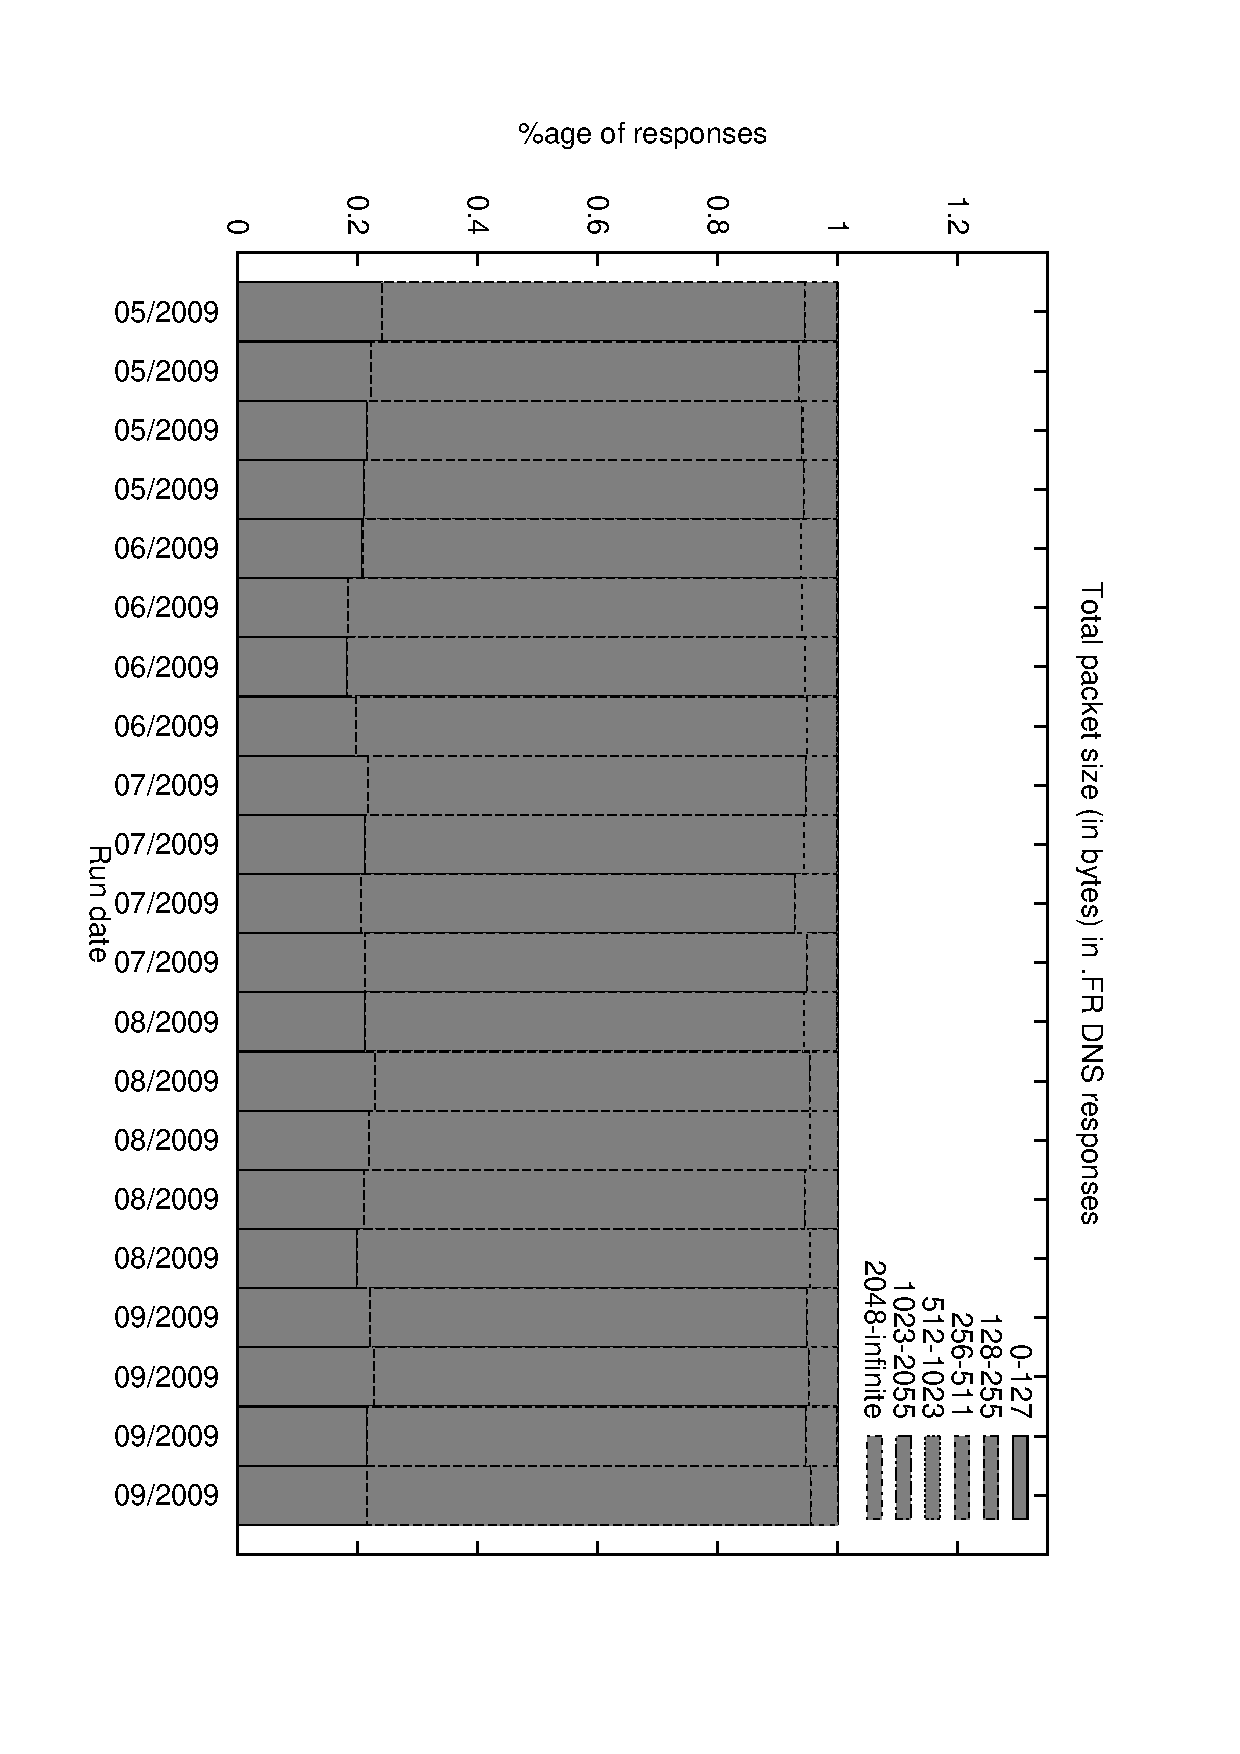
\includegraphics[scale=0.38,angle=90]{respsize.pdf}

.FR does not sign responses yet.
\end{frame}

\begin{frame}
\frametitle{Most queried domains}

\begin{block}
{A important question for the management: what are the most popular
domains?}
{Important, but there are many traps!}
\end{block}

\only<2->{\begin{itemize}
\item Caching at the ISP seriously change the pattern
\item Domains with low TTL are queried more often
\item ``Infrastructure'' domains (used on the right-hand side of the
NS records) are the most popular. If they break, they take many
domains with them.
\end{itemize}}

\only<3->{\dns{nic.fr} is by far the most often queried.}

\only<4->{The ``Top N''study may be published separately. Wait for the
paper :-)}


\end{frame}

\begin{frame}
\frametitle{Kaminsky, one year after}
Still 18 \% of clients without SPR (less than one port per two requests)

They are not only small resolvers, they make 15�\% of the requests.

Methodology: we eliminate small clients (not enough requests) and
recursive requests (dig\ldots).
\end{frame}

\begin{frame}
\frametitle{Percentage of requests per query type}
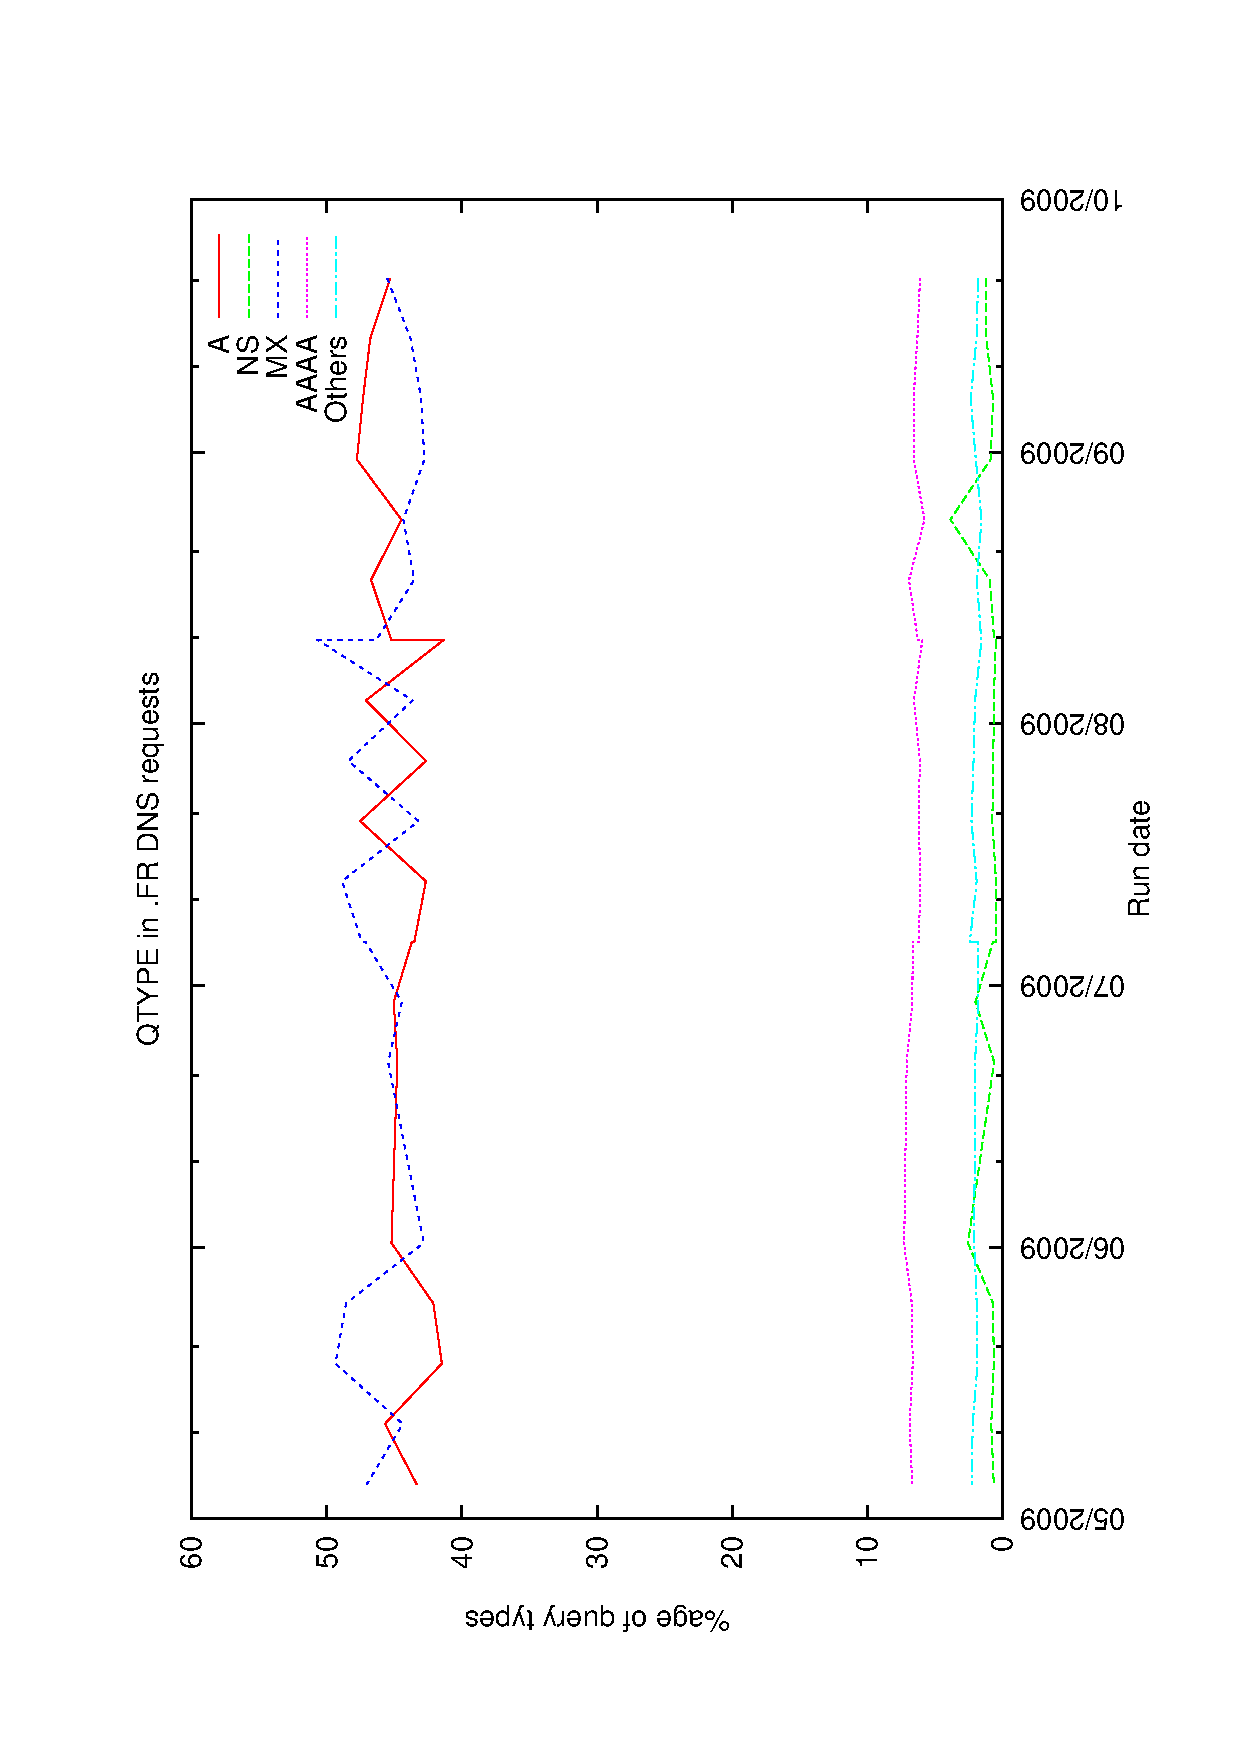
\includegraphics[scale=0.42]{qtypes.pdf}
\end{frame}

\begin{frame}
\frametitle{Comparison with other systems}

\begin{itemize}
\item ISC SIE \url{https://sie.isc.org/}
\item IIS.se dns2db \url{http://opensource.iis.se/trac/dns2db}
\item DSC \url{http://dns.measurement-factory.com/tools/dsc/}
\end{itemize}
\end{frame}

\begin{frame}
\frametitle{DNSmezzo and friends}
\begin{itemize}
\item SIE is optimized for \emph{huge} volumes of data, DNSmezzo for
versatility.
\item DNSmezzo typically works with sampled data (so it requires less
hardware resources but it cannot do security analysis, only stats)
\item DNSmezzo's code is published, we encourage the "perform your
analysis yourself" which can be useful for a TLD.
\item DSC is more targeted to real-time monitoring, its quantitative
precision decreases with time (also, at AFNIC, it is not installed
with QNAME parsing).
\item DNSmezzo is very close, in its principles, to dns2db.
\end{itemize}

\end{frame}

\begin{frame}
\frametitle{Distribution}
\url{http://www.dnswitness.net/}

Distributed under the free software licence GPL.

\end{frame}

\section{Future work}

\begin{frame}
\frametitle{Future work on DNSmezzo}
\begin{itemize}
\item Parse some information that is currently ignored (such as EDNS
option codes, for EDNS0-ping, for instance)
\item Write more reports with the information we have
\item Deploy more probes (warning: consolidation of data from
different name servers is not obvious)
\end{itemize}
\end{frame}

\section{Measurements based on active queries}

\begin{frame}
\frametitle{Active queries}


\only<2>{This is the realm of our \emph{DNSdelve} program.}

\only<3->{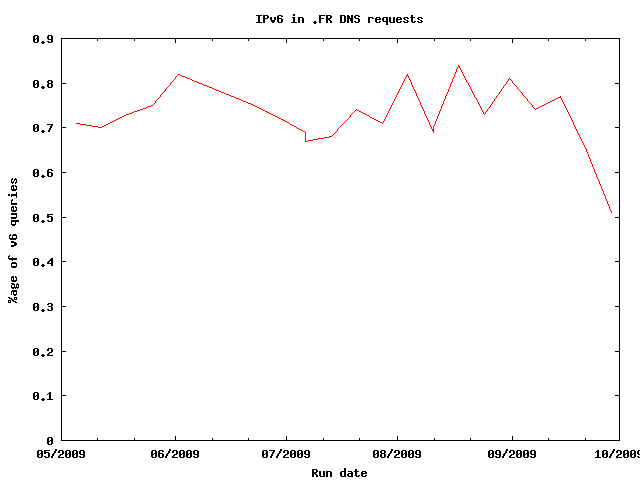
\includegraphics[scale=0.41]{ipv6.pdf}}

\only<4->{Increase but only for name servers. Why?}

\end{frame}

\begin{frame}
\frametitle{Future work on the rest of the project}
\begin{itemize}
\item<1->Gather more users. Yes, you :-)
\item<2->Come back in one year with trends, new applications, etc.
\end{itemize}
\end{frame}

\end{document}
